        \clearpage
        \begin{figure*}[ht]
            \pdfbookmark[2]{ID 07}{figure_id_07}
        	\centering
            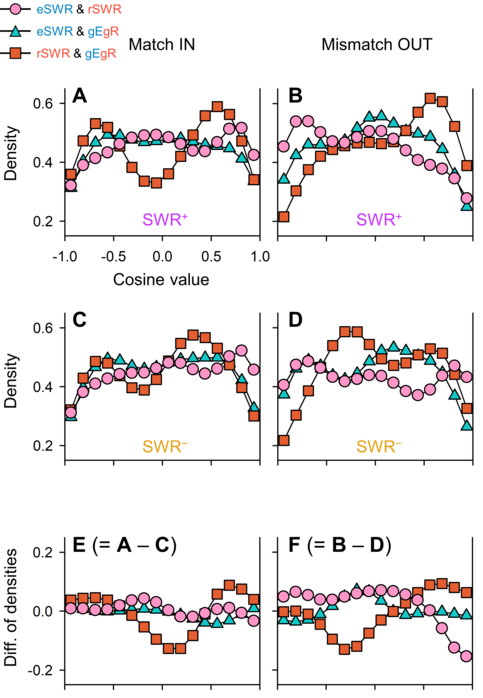
\includegraphics[width=0.5\textwidth]{./src/figures/.png/Figure_ID_07.png}
        	\caption{\textbf{
Analysis of Neural Trajectory Directions during SWR between Encoding, and Retrieval States.
}
\smallskip
\\
\textbf{\textit{A--B}} Kernel density estimation (KDE) distribution of $\protect\overrightarrow{{\mathrm{eSWR^+}}} \cdot \protect\overrightarrow{{\mathrm{rSWR^+}}}$ (\textit{pink circles}), $\protect\overrightarrow{{\mathrm{eSWR^+}}} \cdot \protect\overrightarrow{{\mathrm{g_{E}g_{R}}}}$ (\textit{blue triangles}), and $\protect\overrightarrow{{\mathrm{rSWR^+}}} \cdot \protect\overrightarrow{{\mathrm{g_{E}g_{R}}}}$ (\textit{red rectangles}) in Match In (\textbf{\textit{A}}) and Mismatch OUT task (\textbf{\textit{B}}). \textbf{\textit{C--D.}} The corresponding distributions of $\mathrm{SWR^-}$ in response to those of $\mathrm{SWR^+}$ in \textbf{\textit{A--B}}. \textbf{\textit{E--F.}} The differences in distributions, highlighting the SWR components (\textbf{\textit{E}} = \textbf{\textit{C}} $-$ \textbf{\textit{A}}; \textbf{\textit{F}} = \textbf{\textit{B}} $-$ \textbf{\textit{D}}). Note the inverse directionality between $\protect\overrightarrow{{\mathrm{eSWR^+}}}$ and $\protect\overrightarrow{{\mathrm{rSWR^+}}}$ only in Mismatch OUT task (\textit{pink circles} in \textbf{\textit{E--F}}). Additionally, the shifts from the retrieval to encoding states were observed for SWR components both in Match IN and Mismatch OUT tasks (\textit{red rectangles} in \textbf{\textit{E--F}}).
}
% width=0.5\textwidth
        	\label{fig:07}
        \end{figure*}
